\documentclass[11pt,class=report,crop=false]{standalone}
\usepackage[screen]{../python}


\begin{document}


%====================================================================
\chapitre{Convolution : une dimension}
%====================================================================

\insertvideo{tG93CSTbYfk}{partie 11. Convolution : une dimension}



\objectifs{Ce chapitre permet de comprendre la convolution dans le cas le plus simple d'un tableau à une seule dimension.}

\index{convolution!dimension 1}

%%%%%%%%%%%%%%%%%%%%%%%%%%%%%%%%%%%%%%%%%%%%%%%%%%%%%%%%%%%%%%%%%%%%%
\section{Idée}


La convolution est une opération qui à partir d'un tableau de nombres et d'un motif produit un nouveau tableau de nombres.

\index{convolution!motif}

\myfigure{0.5}{
\tikzinput{fig-convolution1d-01}
}

Le calcul de la liste de sortie se fait par des opérations très simples.
\begin{itemize}
  \item On commence par renverser le motif.
  
  \smallskip
  
\myfigure{0.7}{
\tikzinput{fig-convolution1d-02}
}  
  
  \item On calcule la liste de sortie terme par terme :
  \begin{itemize}
    \item on centre le motif renversé sous la liste d'entrée, à la position à calculer,
    \item on multiplie terme à terme les éléments de la liste d'entrée et ceux du motif,
    \item la somme de tous ces produits est le terme de la liste de sortie.
  \end{itemize}
\end{itemize}



\myfigure{0.7}{
\tikzinput{fig-convolution1d-03}
}



Pour le calcul des coefficients sur les bords, on rajoute des zéros virtuels à gauche et à droite de la liste d'entrée.
\myfigure{0.7}{
\tikzinput{fig-convolution1d-04}
}

\textbf{Notation.} On note $f \conv g$ ce \defi{produit de convolution tronqué}. 
La liste de sortie est de même taille que celle de la liste d'entrée.

\begin{exemple}
Calculons la convolution $[1,0,3,5,1] \conv [1,2,3]$.
On commence par calculer le coefficient le plus à gauche (après ajout d'un zéro virtuel à la liste d'entrée).
\myfigure{0.7}{
\tikzinput{fig-convolution1d-05a}
}
On continue en calculant les coefficients un par un.
\myfigure{0.45}{
\tikzinput{fig-convolution1d-05b}\qquad\qquad
\tikzinput{fig-convolution1d-05c}\qquad\qquad
\tikzinput{fig-convolution1d-05d}\qquad\qquad
\tikzinput{fig-convolution1d-05e}
}

Ainsi  $[1,0,3,5,1] \conv [1,2,3] = [2,6,11,20,17]$.
\end{exemple}



\begin{exemple}
Si le motif est de longueur paire alors on ajoute un $0$ au début du motif pour le calcul.
Ainsi $[-1,5,7,3,2] \conv [4,5] = [-1,5,7,3,2] \conv [0,4,5]$
\myfigure{0.7}{
\tikzinput{fig-convolution1d-06}
}

Lorsque l'on renverse le motif, le zéro ajouté se retrouve à droite !

\myfigure{0.7}{
\tikzinput{fig-convolution1d-07}
}

Après calcul on obtient $[-1,5,7,3,2] \conv [4,5] = [-4, 15, 53, 47, 23]$.

\end{exemple}

%%%%%%%%%%%%%%%%%%%%%%%%%%%%%%%%%%%%%%%%%%%%%%%%%%%%%%%%%%%%%%%%%%%%%
\section{Exemples}

Voyons des exemples de motifs et leur effet sur des tableaux.

\textbf{Moyenne mobile.}
La convolution par le motif $[\frac13,\frac13,\frac13]$ correspond à effectuer une moyenne mobile sur trois termes.

Exemple :
$$[4, 2, 1, 4, 5, 1, 3] \conv \frac13[1,1,1] \simeq [2.00, 2.33, 2.33, 3.33, 3.33, 3.00, 1.33]$$

On peut représenter graphiquement une liste $[x_0,x_1,\ldots,x_N]$ en reliant les points de coordonnées $(k,x_k)$ pour $k$ entre $0$ et $N$. Voici la représentation du tableau d'entrée \couleurnb{en bleu }{}et celle du produit de convolution\couleurnb{ en rouge}{}.
\begin{center}
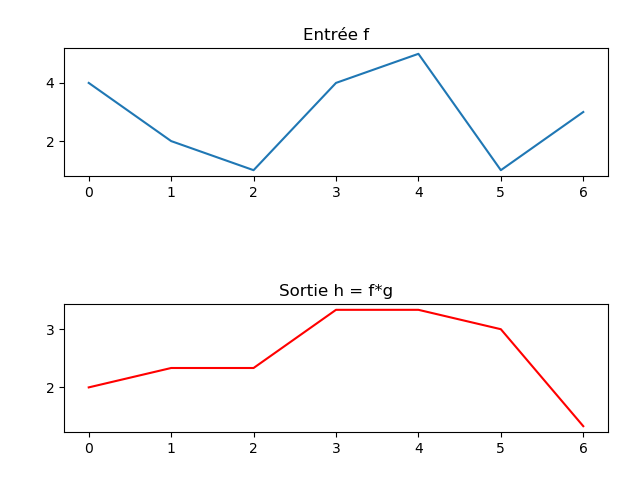
\includegraphics[scale=\myscale,scale=0.6]{figures/convolution-1d-1}
\end{center}

Plus généralement, le motif de longueur $n$ : $\frac1n[1,1,1,\ldots,1]$ correspond à une moyenne mobile sur $n$ termes. Cela permet de \og{}lisser\fg{} des données et de supprimer du \og{}bruit\fg{}.

Exemple :
$$[4, 2, 1, 4, 5, 1, 3] \conv \frac15[1,1,1,1,1] = [1.4, 2.2, 3.2, 2.6, 2.8, 2.6, 1.8]$$


\bigskip

Voici la représentation d'un tableau de $100$ points, au comportement assez chaotique, ainsi que le résultat de son produit de convolution par le motif $\frac13[1,1,1]$ : faire une moyenne mobile \og{}lisse\fg{} la courbe.
 
\begin{center}
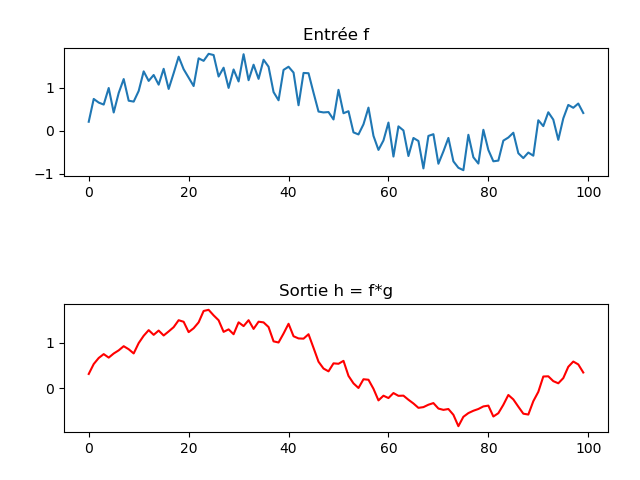
\includegraphics[scale=\myscale,scale=0.6]{figures/convolution-1d-2}
\end{center}

En changeant maintenant le motif de convolution en $\frac15[1,1,1,1,1]$ la courbe est encore plus lisse.

\begin{center}
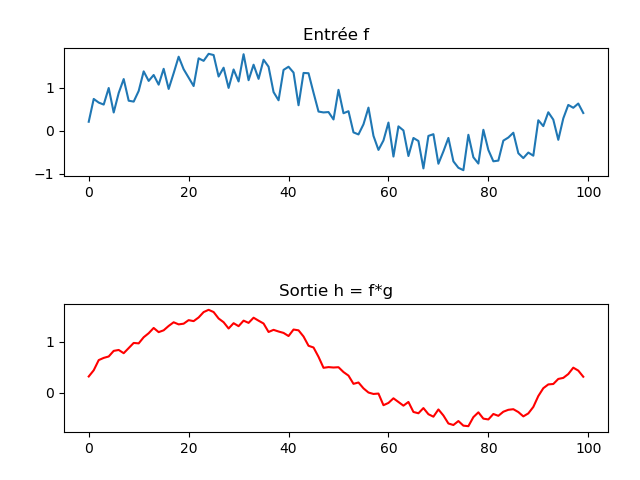
\includegraphics[scale=\myscale,scale=0.6]{figures/convolution-1d-3}
\end{center}

\textbf{Homothétie.}
La convolution par le motif $[k]$ (de longueur $1$ et qui pourrait encore s'écrire $[0,k,0]$) multiplie tous les termes de la liste d'entrée par un facteur $k$.

Exemple :
$$[1,2,3,4,5,6,7,8,9] \conv [2] = [2,4,6,8,10,12,14,16,18].$$


\textbf{Translation.}
La convolution par le motif $[0,0,1]$ décale la liste d'un cran vers la droite (avec ajout d'un zéro en début, le dernier terme disparaissant).

Exemple :
$$[1,2,3,4,5,6,7,8,9] \conv [0,0,1] = [0,1,2,3,4,5,6,7,8].$$


\textbf{Dérivée.}
La convolution par le motif $[0,1,-1]$ (qui s'écrit aussi $[1,-1]$) correspond au calcul de la dérivée de la liste d'entrée vu comme une fonction $n \mapsto f(n)$.

Exemple :
$$[16,9,4,1,0,1,4,9,16]\conv[0,1,-1] = [16, -7, -5, -3, -1,  1,  3,  5,  7].$$
Le calcul correspond à $f(n+1)-f(n)$, une analogie discrète du taux d'accroissement $\frac{f(x+h)-f(x)}{h}$ avec $h=1$.

Pour un tableau d'entrée de $100$ valeurs $[\sin(0),\sin(2\pi/100),\sin(4\pi/100),\ldots,\sin(198\pi/100)]$, définies par la fonction sinus sur $[0,2\pi]$, le produit de convolution par le motif $[0,1,-1]$ donne logiquement un graphe ressemblant au cosinus (à un facteur multiplicatif près).
\begin{center}
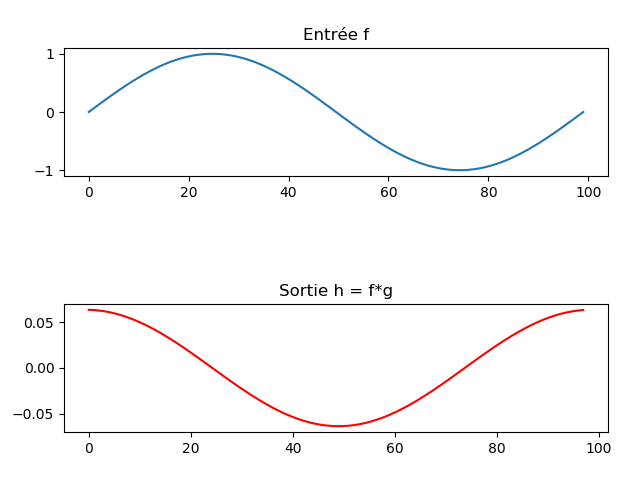
\includegraphics[scale=\myscale,scale=0.6]{figures/convolution-1d-4}
\end{center}


On retient donc que la convolution par un motif, peut rendre la liste plus lisse, la transformer (homothétie, translation) et peut en extraire certaines propriétés (comme la dérivée).


%%%%%%%%%%%%%%%%%%%%%%%%%%%%%%%%%%%%%%%%%%%%%%%%%%%%%%%%%%%%%%%%%%%%%
\section{Réseau de neurones}

\index{convolution!couche de neurones}

Comment créer un nouveau type de réseau de neurones réalisant un produit de convolution ?
Nous allons créer un nouveau type de neurone et un nouveau type de couche de neurones correspondant à un motif donné.

Pour un motif  $[a,b,c]$, un neurone de convolution possède trois arêtes, de poids $a,b,c$, et est relié à seulement trois valeurs de l'entrée.


\myfigure{0.6}{
\tikzinput{fig-convolution1d-08}
}

La sortie est $s=xc+yb+za$. On pourrait aussi composer par une fonction d'activation $\phi$, auquel cas la sortie serait $s=\phi(xc+yb+za)$.

On peut représenter une couche de convolution par un ensemble de neurones de convolution, 
ceux-ci ayant tous les mêmes poids $[a,b,c]$ et chacun étant relié à seulement trois valeurs de l'entrée. La sortie produite est alors le produit  convolution de l'entrée par le motif $[a,b,c]$.
Pour une entrée de longueur $n$, la couche de convolution possède $n$ neurones, chaque neurone ayant trois arêtes (sauf les neurones de bord). Mais au total, il n'y a que trois poids différents.


\myfigure{1}{
\tikzinput{fig-convolution1d-09}
}

Quel est l'avantage de cette couche de neurones par rapport à une couche complètement connectée (comme dans les chapitres précédents) ?
Dans une couche complètement connectée de $n$ neurones ayant une entrée de taille $n$, il y a $n^2$ coefficients alors qu'ici il n'y a que $3$ coefficients (quel que soit $n$). Par exemple, si $n=100$ alors il y a seulement $3$ coefficients à calculer au lieu de $10\,000$.


\myfigure{1}{
\tikzinput{fig-convolution1d-10}\qquad\qquad\qquad\qquad
\tikzinput{fig-convolution1d-11}
}
Sur la figure du gauche, nous avons une couche complètement connectée à la précédente. Chaque arête correspond à un poids à calculer. Sur la figure de droite, une couche de convolution (de taille $3$) est connectée à la précédente.
Chaque neurone n'a que $3$ arêtes (sauf les neurones extrêmes qui n'en ont que deux) et de plus les arêtes partagent leur poids (les arêtes rouges ont toutes le même poids $a$, les arêtes vertes le même poids $b$, les arêtes bleues le même poids $c$).


%%%%%%%%%%%%%%%%%%%%%%%%%%%%%%%%%%%%%%%%%%%%%%%%%%%%%%%%%%%%%%%%%%%%%
\section{Définition mathématique}

Cette partie  n'est pas utile pour les chapitres suivants, mais présente les choses de façon plus théorique.
En particulier, il n'y a plus à ajouter de zéros virtuels (ni sur la liste d'entrée, ni sur un motif de longueur paire). 


\begin{definition}
Soient $(f(n))_{n\in\Zz}$ et $(g(n))_{n\in\Zz}$ deux suites de nombres réels.
Le \defi{produit de convolution} $f \fullconv g$ est la suite $(h(n))_{n\in\Zz}$ dont le terme général est défini par :
\mybox{$\displaystyle f \fullconv g(n) = \sum_{k=-\infty}^{+\infty} f(n-k) \cdot g(k)$}
\end{definition}

Il ne faut pas avoir peur de cette formule. En particulier, dans les situations rencontrées ici, il n'y a pas vraiment une infinité de termes à calculer. Voici une formule plus simple, lorsque l'on suppose que les termes de $g$ sont nuls en dehors des indices appartenant à $[-K,+K]$ :

\mybox{$\displaystyle f \fullconv g(n) = \sum_{k=-K}^{+K} f(n-k) \cdot g(k)$}


Reprenons l'exemple de la convolution de $[1,0,3,5,1]$ par $[1,2,3]$.
Choisissons $(f(n))_{n\in\Zz}$  la suite dont les termes non tous nuls sont $[f(0)=1,f(1)=0,f(2)=3,f(3)=5,f(4)=1]$
et choisissons $(g(n))_{n\in\Zz}$ la suite dont les termes non tous nuls sont $[g(-1)=1,g(0)=2,g(1)=3]$. 
% Il existe une infinité de définitions possibles pour les suites $f$ et $g$, le choix a été fait ici de positionner le premier élément de la liste au rang $0$ pour $f$ et au rang $-1$ pour $g$.
Alors on obtient la convolution $h = f \fullconv g$ par la formule ci-dessus : 
$$f \fullconv g (n) = \sum_{k=-1}^{+1} f(n-k) \cdot g(k) = f(n-1)g(1) + f(n)g(0) +f(n+1)g(-1).$$

On retrouve la méthode pratique vu précédemment : on renverse le motif $g$ avant de faire une série de multiplications.
Par exemple $f \fullconv g (1) = f(0)g(1) + f(1)g(0) +f(2)g(-1) = 1\times 3 + 0\times2 + 3\times 1=6$.
 

\myfigure{0.8}{
\tikzinput{fig-convolution1d-12}
}

Le résultat de la convolution est la suite 
$$[ \ldots, 0, 0, 1,  2,  6, 11, 20, 17,  3, 0 , 0, \ldots]$$
où le terme de rang $0$ est $f \fullconv g(0) = 2$. Ce résultat est indépendant, à un décalage près, des choix opérés dans les définitions de $f$ et $g$.


La convolution tronquée consiste à ne retenir qu'une sous-liste de même taille que la liste d'entrée en tronquant les bords (la façon de tronquer dépend du choix des définitions de $f$ et $g$). Ainsi : 
$[1,0,3,5,1] \conv [1,2,3]= [2,  6, 11, 20, 17]$.

\myfigure{0.8}{
\tikzinput{fig-convolution1d-13}
}


Terminons par une propriété remarquable du produit de convolution.
En réindexant la somme de la définition, on obtient :
$$f \fullconv g(n) = \sum_{k=-\infty}^{+\infty} f(k) \cdot g(n-k).$$
Ce qui signifie que le produit de convolution est symétrique : 
\mybox{$\displaystyle f \fullconv g(n) = g \fullconv f(n)$}


\begin{remarque*}
\sauteligne
\begin{itemize}
  \item La convolution est très utilisée en théorie du signal, c'est pourquoi on trouve aussi le vocabulaire \emph{signal d'entrée}, \emph{signal de sortie}. C'est aussi pour des raisons de signal qu'on renverse une des listes avant de faire les multiplications.
  
  \item Le \defi{motif} s'appelle aussi \defi{noyau} (\emph{kernel} en anglais) mais aussi \defi{masque} ou \defi{filtre}.
\end{itemize}
\end{remarque*}

\end{document}
